\section{Experimental Development}

\subsection{Preprocessing and Segmentation}

All images were resized to $224 \times 224$ pixels before being used by the CNN, segmentation module, or handcrafted feature extractor. For the segmentation-based scenarios, each RGB image was converted to the L*a*b* color space. The binary region-of-interest mask was generated from the $a$ channel using Otsu thresholding \cite{otsu1979threshold}. This channel was selected because it captures the green-red chromatic component, which is useful for separating leaf and lesion regions from parts of the background.

The resulting binary mask was refined using morphological opening and closing with a kernel size of 5. Pixels outside the mask were replaced by zero, producing a segmented image. Given an input image $I$ and a binary mask $M$, the segmented image $I_s$ was computed as:

\begin{equation}
I_s(x,y) =
\begin{cases}
I(x,y), & \text{if } M(x,y)=1,\\
0, & \text{otherwise.}
\end{cases}
\end{equation}

This segmentation strategy was used for E1 and E3. In E1, the segmented image was passed directly to MobileNetV2. In E3, the segmented image was used both as CNN input and as the source for extracting handcrafted texture and frequency features.

\subsection{Texture Feature Extraction}

Explicit handcrafted descriptors were extracted from original images for E2 and from segmented images for E3. The feature extractor combined gray-level co-occurrence matrix (GLCM) descriptors and discrete wavelet transform (DWT) descriptors.

The GLCM descriptors represented spatial gray-level relationships using contrast, dissimilarity, homogeneity, energy, correlation, and angular second moment (ASM) \cite{haralick1973glcm}. For each descriptor, the mean and standard deviation were computed, producing 12 texture features.

The DWT descriptors represented multiresolution frequency information \cite{mallat1989wavelet}. Mean, standard deviation, energy, and entropy were extracted from the approximation coefficients and from horizontal, vertical, and diagonal detail coefficients at two decomposition levels. This produced 28 frequency-domain features. Therefore, each image used in the texture-based scenarios was represented by 40 numerical handcrafted descriptors: 12 GLCM-based features and 28 DWT-based features.

Before training the hybrid models, the handcrafted feature vectors were standardized using a \texttt{StandardScaler}. The scaler was fitted only on the training split and then applied to the validation and test splits, preventing information leakage during normalization.

\subsection{Model Architecture}

The image backbone was MobileNetV2 with ImageNet pre-trained weights \cite{sandler2018mobilenetv2}. For E0 and E1, the original classifier head was replaced by a dropout layer followed by a fully connected layer with four output units, corresponding to the four disease classes. The backbone was fine-tuned during training.

For E2 and E3, a two-branch hybrid architecture was implemented. The first branch extracted an image embedding using MobileNetV2 followed by adaptive average pooling. The second branch processed the standardized 40-dimensional handcrafted feature vector through a fully connected layer with 128 hidden units, ReLU activation, and dropout. The image embedding and texture representation were concatenated and passed to a fusion classifier with 256 hidden units, ReLU activation, dropout, and a final four-class output layer.

Figure~\ref{fig:proposed_hybrid_architecture} illustrates the proposed E3 architecture. In this configuration, the segmented image is used both as the CNN input and as the source for explicit GLCM+DWT feature extraction, making the fusion between segmentation and handcrafted descriptors explicit.

\begin{figure}[!t]
\centering
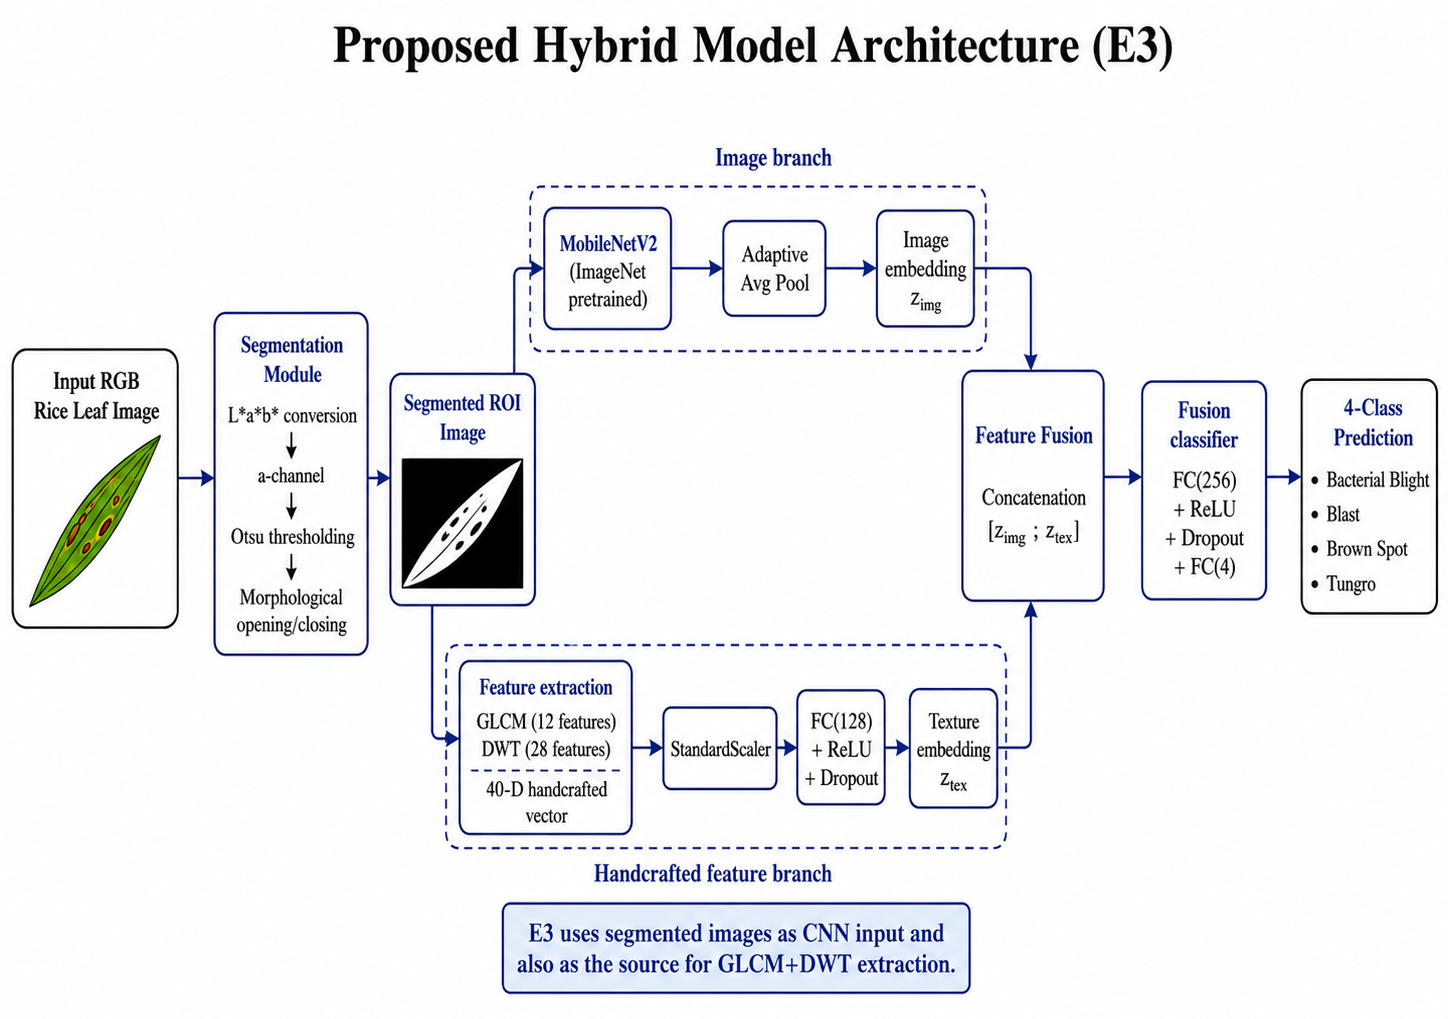
\includegraphics[width=\columnwidth]{figures/fig02_proposed_hybrid_architecture_e3.png}
\caption{Proposed hybrid model architecture for E3.}
\label{fig:proposed_hybrid_architecture}
\end{figure}

Let $\mathbf{z}_{img}$ denote the MobileNetV2 image embedding and $\mathbf{z}_{tex}$ denote the learned representation of the handcrafted feature vector. The fused representation is defined as:

\begin{equation}
\mathbf{z}_{fused} = [\mathbf{z}_{img}; \mathbf{z}_{tex}],
\end{equation}

where $[\,;\,]$ denotes vector concatenation. The final class prediction is obtained by applying the fusion classifier to $\mathbf{z}_{fused}$.


\subsection{Training Configuration and Implementation Details}

All models were trained with the same configuration: 30 maximum epochs, batch size of 8, AdamW optimizer, learning rate of $1 \times 10^{-4}$, weight decay of $1 \times 10^{-4}$, cosine learning-rate scheduler, and early stopping with patience of 7 based on validation macro-F1.

The implementation was developed in Python using PyTorch for model training, OpenCV for image processing and segmentation, scikit-image and PyWavelets for feature extraction, and scikit-learn for feature standardization and evaluation utilities. The experiments were executed on an NVIDIA GeForce RTX 3050 Laptop GPU with CUDA support.